\par Para este segundo experimento tomamos nuestras mediciones en una red WIFI laboral durante una hora.

\subsubsection{Fuente $S$}

\par Veamos entonces las m\'etricas de la fuente $S$ propuesta modelada con los resultados del experimento: \\

\begin{tabular}{ | c | c | c |}
    \hline
    Mensaje & Probabilidad & Información [bits] \\
    \hline
    \textit{Unicast} & 0.464 & 1.109 \\
    \hline
    \textit{Broadcast} & 0.536 & 0.898 \\
    \hline
\end{tabular} \\

\par Entropía de la fuente: 0.996 bits. Entropía máxima: 1 bit.

\par En este caso podemos observar como las probabilidades de aparici\'on de los dos tipos de paquetes rondan el 50\%, es decir, sus apariciones son pr\'acticamente equiprobables. \\
De esto podemos deducir y comprobar matem\'aticamente que los simbolos de la fuente $S$ casi no nos brindan informaci\'on. Por tal m\'otivo, si observamos la entrop\'ia de la misma, vamos a notar que se acerca demasiado a 1 bit, es decir, la entrop\'ia m\'axima, lo cual tiene sentido ya que sabemos que este valor se alcanza cuando los eventos son equiprobables, y en nuestro caso, las apariciones de los simbolos de $S$ se asemejan mucho a ese escenario.

\par Algo que nos llam\'o poderosamente la atenci\'on en esta red es que m\'as de la mitad de los paquetes hayan sido env\'iados como broadcast, habiendo captado durante la hora de medici\'on 4641 paquetes de tipo broadcast y 4013 de tipo unicast. \\
Por tal m\'otivo decidimos analizar un poco m\'as en profundidad qu\'e es lo que estaba sucediendo con los paquetes enviados como broadcast.

Lo primero que hicimos fue mapear por los tipos de paquetes, obteniendo los siguientes resultados:

\begin{figure*}[ht]
    \centering
    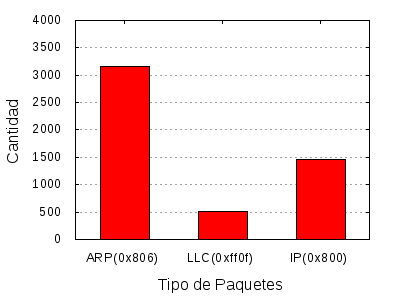
\includegraphics[scale=0.7]{figuras/experimento2-tipos-paquetes.png}
    \caption{Tipos de paquetes broadcast.}\label{Tipos de paquetes}
\end{figure*}

Como podemos observar en la figura ??, la mayor cantidad de paquetes son de tipo ARP. Tambi\'en podemos notar una cantidad m\'inima de paquetes de tipo LLC (Logical Link Control). Este paquete es propio del estandard IEEE 802.2 que define el control de enlace l\'ogico para redes de \'area local en el modelo OSI. Estos dos tipos de paquetes son utilizados por protocolos de control y su funcionamiento requiere del env\'io de paquetes broadcast. Lo que nos llam\'o la atenci\'on aqu\'i es la gran cantidad de paquetes de tipo IP que hallamos.

Decidimos entonces profundizar en este punto y tratar de entender que pasaba con estos paquetes IP env\'iados a todos los nodos. \\
Para esto, graficamos la cantidad de paquetes de este tipo enviados por IP de origen, como se puede ver en la figura ??:

\begin{figure*}[ht]
    \centering
    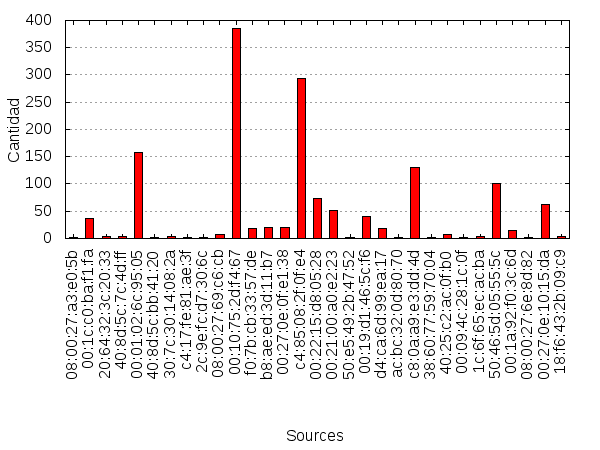
\includegraphics[scale=0.7]{figuras/experimento2-ips-origen.png}
    \caption{Sources de paquetes IP broadcast.}\label{Sources de paquetes IP broadcast}
\end{figure*}

Observemos de los paquetes de tipo IP que emiten un broadcast, los tres primeros sources que sobresalen del resto en cuanto a cantidad de paquetes enviados. Estos son los nodos cuyas MAC adreess son: 00:10:75:2d:f4:67 (386 paquetes), c4:85:08:2f:0f:e4 (294 paquetes) y 00:01:02:6c:95:05 (157 paquetes).
Por lo tanto, al analizar los paquetes que provenían de estos nodos en modo broadcast y que son de tipo IP, encontramos que emitían los siguientes mensajes:

\begin{itemize}
	\item 00:10:75:2d:f4:67	: Hello there. I am at 192.168.1.120. Time is 1474050708 and I am hungry.Hostname: backupdyd.seagateshare.com \\
		Lo que notamos ac\'a es que se trata de un software de backup que podr\'ia estar notificando a todos los nodos sus datos para posteriores procesos.
	\item c4:85:08:2f:0f:e4	: De este source no pudimos obtener mucha informaci\'on como para poder determinar el por qu\'e del env\'io de paquetes broadcast.
	\item 00:01:02:6c:95:0: 9016 3 ipp://192.168.1.150:631/printers/HP-LaserJet-P1006 "" "HP LaserJet P1006" "HP LaserJet P1006 Foomatic/foo2xqx (recommended)" job-shee    ts=none,none lease-duration=300 \\
		En este caso, se trata de mensajes emitidos por impresoras que eventualmente podr\'ian querer informar sus status a todos los nodos.
\end{itemize}

Por lo tanto, podemos conclu\'ir aqu\'i que se trata de paquetes para control pero no de la red en si misma, sino de protocolos propios de ciertos nodos.